\chapter{Resultados e Discussão}\label{cap:resultados}

O primeiro teste foi executado como agente percorrendo somente um percurso, este que possui uma dificuldade mediana, o agente apenas precisa fazer uma curva a esquerda.

\begin{figure}[h]
    \centering
    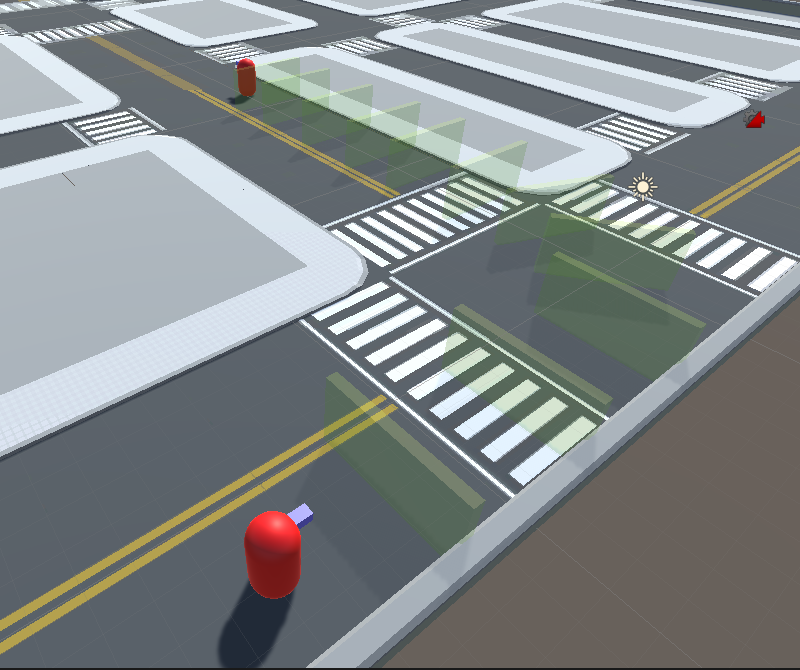
\includegraphics[scale=0.35]{figs/rotas/path_1.png}
     \caption{O percurso executado no primeiro treino. A cápsula vermelha em baixo indica a posição inicial do veículo e a na parte superior indica o destino.}
     \label{fig:rota-1}
  \end{figure}
 
Após completar o treino o desempenho do agente 

\section{Base de Dados}

\lipsum[72]

\section{Considerações Finais}

\lipsum[74]